%%%%%%%%%%%%%%%%%%%%%%%%% NOTE %%%%%%%%%%%%%%%%%%%%%%%%%%%%
%% You can ignore everything from here until             %%
%% "Question 1: Introduction"                            %%
%%%%%%%%%%%%%%%%%%%%%%%%%%%%%%%%%%%%%%%%%%%%%%%%%%%%%%%%%%%
\documentclass[8pt]{article}
\usepackage{amsmath, amsfonts, amsthm, amssymb}  % Some math symbols
\usepackage{fullpage}
\usepackage{graphicx}
\usepackage[x11names, rgb]{xcolor}
\usepackage{graphicx}
\usepackage{tikz}
\usetikzlibrary{decorations,arrows,shapes}

\usepackage{etoolbox}
\usepackage{enumerate}
\usepackage{listings}

\setlength{\parindent}{0pt}
\setlength{\parskip}{5pt plus 1pt}

\newcommand{\N}{\mathbb N}
\newcommand{\E}{\mathbb E}
\newcommand{\V}{Var}
\renewcommand{\P}{\mathbb P}
\newcommand{\f}{\frac}


\newcommand{\nopagenumbers}{
    \pagestyle{empty}
}

\def\indented#1{\list{}{}\item[]}
\let\indented=\endlist

\providetoggle{questionnumbers}
\settoggle{questionnumbers}{true}
\newcommand{\noquestionnumbers}{
    \settoggle{questionnumbers}{false}
}

\newcounter{questionCounter}
\newenvironment{question}[2][\arabic{questionCounter}]{%
    \addtocounter{questionCounter}{1}%
    \setcounter{partCounter}{0}%
    \vspace{.25in} \hrule \vspace{0.4em}%
        \noindent{\bf \iftoggle{questionnumbers}{#1: }{}#2}%
    \vspace{0.8em} \hrule \vspace{.10in}%
}{$ $\newpage}

\newcounter{partCounter}[questionCounter]
\renewenvironment{part}[1][\alph{partCounter}]{%
    \addtocounter{partCounter}{1}%
    \vspace{.10in}%
    \begin{indented}%
       {\bf (#1)} %
}{\end{indented}}

\def\show#1{\ifdefempty{#1}{}{#1\\}}

\newcommand{\header}{%
\begin{center}
    {\Large \show\myhwname}
    \show\myname
    \show\myemail
    \show\mysection
    \show\hwname
\end{center}}

\usepackage{hyperref} % for hyperlinks
\hypersetup{
    colorlinks=true,
    linkcolor=blue,
    filecolor=magenta,      
    urlcolor=blue,
}

%%%%%%%%%%%%%%%%% Identifying Information %%%%%%%%%%%%%%%%%
%% For 312, we'd rather you DIDN'T tell us who you are   %%
%% in your homework so that we're not biased when        %%
%% So, even if you fill this information in, it will not %%
%% show up in the document unless you uncomment \header  %%
%% below                                                 %%
%%%%%%%%%%%%%%%%%%%%%%%%%%%%%%%%%%%%%%%%%%%%%%%%%%%%%%%%%%%
\newcommand{\myhwname}{DS288 (AUG) 3:0 Numerical Methods }
\newcommand{\myname}{Naman Pesricha }
\newcommand{\myemail}{namanp@iisc.ac.in}
\newcommand{\hwname}{\textbf{Homework-1}}
\newcommand{\mysection}{SR - 24115}
%%%%%%%%%%%%%%%%%%%%%%%%%%%%%%%%%%%%%%%%%%%%%%%%%%%%%%%%%%%

%%%%%%%%%%%%%%%%%%% Document Options %%%%%%%%%%%%%%%%%%%%%%
\noquestionnumbers
\nopagenumbers
%%%%%%%%%%%%%%%%%%%%%%%%%%%%%%%%%%%%%%%%%%%%%%%%%%%%%%%%%%%

\begin{document}
\header
\hline


A Microwave engineer is interested in developing a hazardous waste treatment facility based on
microwave exposure to the hazardous material. The design is based on cylindrical microwave
cavity and requires computing of various modes of the electromagnetic fields that will exist in
this structure. The modes of the systems are described by the Bessel functions $J_i(x)$ for i =
1,2, ... , n. As a numerical methods expert, your job is to help the engineer to compute these
Bessel functions using the recurrence relation
\begin{equation}
J_{n-1}(x) + J_{n+1}(x) = \frac{2n}{x}J_n(x)
\end{equation}

\begin{table}[h!]
\centering
\begin{tabular}{c c c c}
\hline
$n$ & $J_n(1)$ & $J_n(5)$ & $J_n(50)$ \\
\hline
0  & $7.6519768656 \times 10^{-1}$ & $-1.7759677131 \times 10^{-1}$ & $5.5812327669 \times 10^{-2}$ \\
1  & $4.4005058574 \times 10^{-1}$ & $-3.2757913759 \times 10^{-1}$ & $-9.7511828125 \times 10^{-2}$ \\
2  & $1.1490348493 \times 10^{-1}$ & $4.6565116278 \times 10^{-2}$ & $-5.9712800794 \times 10^{-2}$ \\
3  & $1.9563353983 \times 10^{-2}$ & $3.6483123061 \times 10^{-1}$ & $9.2734804062 \times 10^{-2}$ \\
4  & $2.4766389641 \times 10^{-3}$ & $3.9123236046 \times 10^{-1}$ & $7.0840977282 \times 10^{-2}$ \\
5  & $2.4975773021 \times 10^{-4}$ & $2.6114054612 \times 10^{-1}$ & $-8.1400247697 \times 10^{-2}$ \\
6  & $2.0938338002 \times 10^{-5}$ & $1.3104873178 \times 10^{-1}$ & $-8.7121026821 \times 10^{-2}$ \\
7  & $1.5023258174 \times 10^{-6}$ & $5.3376410156 \times 10^{-2}$ & $6.0491201260 \times 10^{-2}$ \\
8  & $9.4223441726 \times 10^{-8}$ & $1.8405216655 \times 10^{-2}$ & $1.0405856317 \times 10^{-1}$ \\
9  & $5.2492501799 \times 10^{-9}$ & $5.5202831385 \times 10^{-3}$ & $-2.7192461044 \times 10^{-2}$ \\
10 & $2.6306151237 \times 10^{-10}$ & $1.4678026473 \times 10^{-3}$ & $-1.1384784915 \times 10^{-1}$ \\
\hline
\end{tabular}
\caption{Bessel functions of integer order (n = 0 - 10) for x = 1, 5, and 50.}
\label{tab:jn_values}
\end{table}




\begin{question}{Q1 Compute the recursion in the forward direction, i.e., compute $J_2(x)$ from $J_1(x)$ and $J_0(x)$
with starting values taken from the table-1. Use only the first 5 digits given in the table
for each quantity when supplying the starting values to your program. For x = 1,5, and
50, how accurate is $J_{10}(x)$ ?. Compute both the absolute and relative errors of these values
taking the tabulated values (table-1) as truth. [3 points]}
\textbf{Answer:} We will initialize the first two rows ( $J_0(x)$ and $J_1(x)$ ) from values from the table using only the first 5 digits and compute forward.
- Iterative scheme rearranged for forward computation: 
\begin{equation}
    J_n(x) = \frac{2(n-1)}{x}J_{n-1}(x) - J_{n-2}(x)
\end{equation}
    
- Absolute error can be calculated using: $$|(data - \hat{data})|$$
- Relative error can be calculated using: $$|\frac{(data - \hat{data})}{data}|$$

\begin{table}[h!]
\centering
\begin{tabular}{c c c c}
\hline
 & $J_{10}(1)$ & $J_{10}(5)$ & $J_{10}(50)$ \\
\hline
ActualValue    & $2.6306151237 \times 10^{-10}$ & $1.4678026473 \times 10^{-3}$ & $-1.1384784915 \times 10^{-1}$ \\
ComputedValue  & $5.6055331000 \times 10^{2}$   & $1.5852559616 \times 10^{-3}$ & $-1.1384696301 \times 10^{-1}$ \\
AbsoluteError  & $5.6055331000 \times 10^{2}$   & $1.1745331430 \times 10^{-4}$ & $8.8613829735 \times 10^{-7}$ \\
RelativeError  & $2.1308830203 \times 10^{12}$  & $8.0019827270 \times 10^{-2}$ & $-7.7835313005 \times 10^{-6}$ \\
\hline
\end{tabular}
\caption{Comparison of Actual, Computed Values, and Errors for $J_{10}(x)$ in forward computation.}
\label{tab:j10_values}
\end{table}

\begin{figure}[ht]
    \centering
    \begin{minipage}{0.7\textwidth}
        \centering
        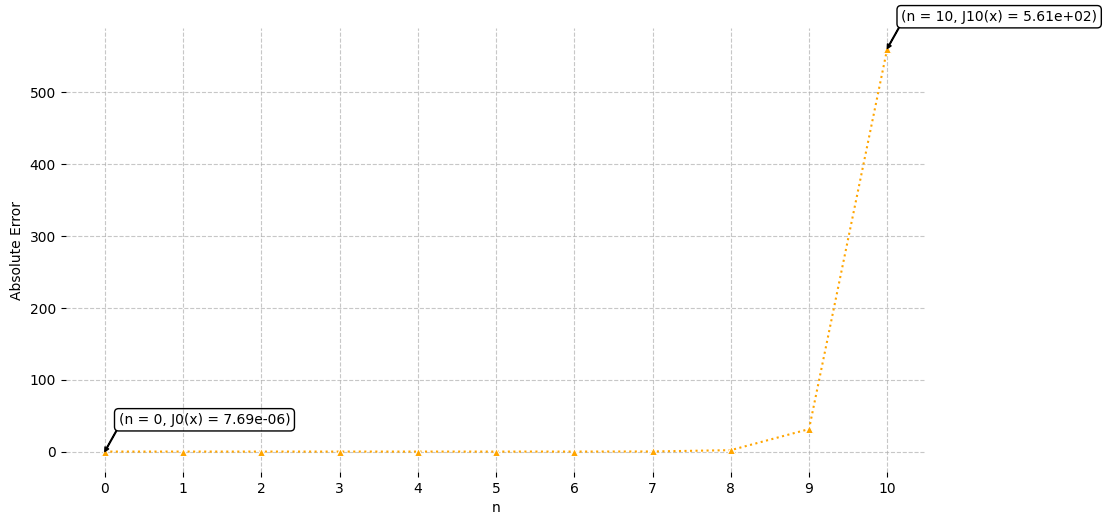
\includegraphics[width=\textwidth]{FW1.png} % Replace with your figure file
        \caption{Forward Absolute Error for x = 1}
        \label{fig:your-label}
    \end{minipage}%
    \begin{minipage}{0.3\textwidth}
        \centering
        \textbf{Observation 1:} \\ The error in forward pass grew from order of $10^{-6}$ to order of $10^{-12}$.
        
    \end{minipage}
\end{figure}

\begin{figure}[ht]
    \centering
    \begin{minipage}{0.7\textwidth}
        \centering
        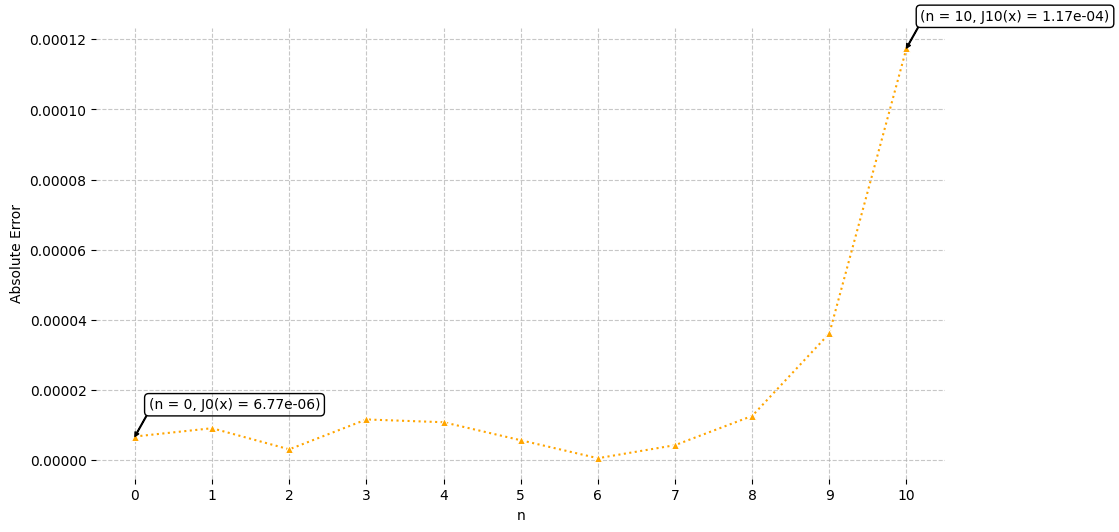
\includegraphics[width=\textwidth]{FW5.png} % Replace with your figure file
        \caption{Forward Absolute Error for x = 5}
        \label{fig:your-label}
    \end{minipage}%
    \begin{minipage}{0.3\textwidth}
        \centering
        \textbf{Observation 2:} \\
        The error growth for x = 5 for forward pass seems to be exponential at around from n = \{6 to 10\}.
        The error in forward pass grew from order of $10^{-6}$ to order of $10^{-4}$.
    \end{minipage}
\end{figure}

\begin{figure}[ht]
    \centering
    \begin{minipage}{0.7\textwidth}
        % \centering
        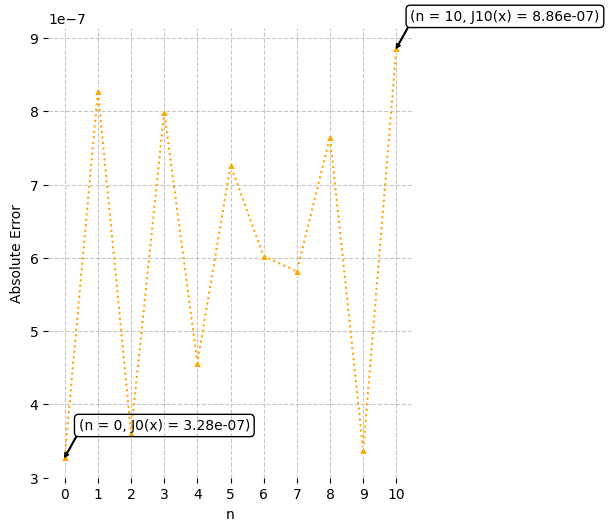
\includegraphics[width=\textwidth]{FW50.png} % Replace with your figure file
        \caption{Forward Absolute Error for x = 50}
        \label{fig:your-label}
    \end{minipage}%
    \begin{minipage}{0.3\textwidth}
        % \centering
        \textbf{Observation 3: } \\
        
    \end{minipage}
\end{figure}



\end{question}


% \begin{question}{Problem 2 (multi-part example, and large numbers)}

% \begin{part}

% \textbf{Answer:} \fbox{$20! \cdot \binom{13}{5} \approx 3.131 \cdot 10^{21}$}

% (Please give the raw formula you used, \textbf{and} its value, possibly in scientific notation if it is too
% large).


% \textbf{Explanation:}

% Explain here.
% \end{part}

% \begin{part}

% \textbf{Answer:} \fbox{$answer$}

% \textbf{Explanation:} 

% Explain here.

% \end{part}

% \end{question}
% \begin{question}{Problem 3 (proof problem example)} 

% \textbf{(Short way)}

% You can use the \textbf{align*} environment to align a proof or
% calculation. Example below: 

% \begin{align*}
%     \P(E|F) &= \dfrac{\P(E \cap F)}{\P(F)}     & \text{(def of conditional probability)} \\
%             &= \dfrac{\P(F|E) \P(E)}{\P(F)}    & \text{(chain rule)}
% \end{align*}


% \textbf{How did I produce that?} The ``align*'' environment produces a table structure. You use \& to go to the next ``column'', and \text{\textbackslash \textbackslash} to start a new line. The whitespaces in the .tex document were not necessary. \\

% \textbf{(Long way)}

% First, by the chain rule, we have
% $$\P(E|F) \P(F) = \P(E \cap F)$$

% Switching the roles of $E$ and $F$ gives
% $$\P(F|E) \P(E) = \P(F \cap E)$$

% Since $\P(E \cap F) = \P(F \cap E)$, we can set them equal to get
% $$\P(E|F) \P(F) = \P(F|E) \P(E)$$

% But dividing by $\P(F) > 0$ gives Bayes Theorem
% $$\P(E|F) = \dfrac{\P(F|E) \P(E)}{\P(F)}$$
% \end{question}

% \begin{question}{Problem 4 (Calculus notation)}
% \begin{part} The syntax for integrals, summations, etc is a bit clunky but should be intuitive.

% $$ \int_{a}^{b}{f(x)dx} $$

% $$ \sum_{i=1}^{n} X_i $$

% $$ \prod_{i=1}^{n} \P(x_i | \theta) $$

% \end{part}
% \begin{part} Partial derivatives:
% $$ \dfrac{\partial}{\partial \theta} L(x_1, x_2, \dots x_n | \theta) = 2x$$

% \end{part}
% \end{question}

\end{document}
